% tutorial_example_attenuation.tex — worked example: attenuation correction.
% Standalone document; reuses recocrysp_tutorial.sty and the shared bibliography
% (tbsrc/references). Refers to the Foundations tutorial (Part I) by name. The
% runnable code lives in tutorial/examples/attenuation/.
%
% Build (from this directory):  make   (builds the basis first, then this)
\documentclass[11pt,a4paper]{article}
\usepackage{recocrysp_tutorial}

\title{RecoCrysp Tutorial\,---\,Worked Example\\[2pt]
       \large Attenuation Correction}
\author{J.~J.~G\'omez-Cadenas}
\date{\today}

\begin{document}
\maketitle

\begin{abstract}
A first worked example with \code{RecoCrysp}: a uniform-activity water sphere on
a continuous (CRYSP) scanner. We simulate attenuated, Poisson-noisy listmode
data and reconstruct it with and without attenuation correction, reproducing the
classic cupping artifact and its removal. The example uses only the projectors
and the listmode MLEM of the Foundations tutorial (Part~I); detector resolution
is switched off here and added in a later example. The runnable code is in
\code{tutorial/examples/attenuation/}.
\end{abstract}

\section{Overview}
\label{sec:ex-att:overview}

Attenuation is the dominant quantitative effect in PET: a coincidence survives
only if both $511\,\mathrm{keV}$ photons escape the body, so lines of response
through more material record fewer counts. Ignored, this depresses the
reconstructed activity towards the centre of the object --- the \emph{cupping}
artifact. This example demonstrates the effect and its correction on the
simplest revealing phantom, a uniform sphere of water.

It exercises exactly the data model of Part~I (the Data Model section): with
normalization $\nrm=\bm1$, no background ($\sct=\rnd=\bm0$), and detector
resolution switched off ($\Gop=\mathbf I$), the mean counts on LOR $i$ reduce to
\begin{equation}
  \pred_i \;=\; a_i\,(\Aop\,\xv)_i ,
  \qquad
  a_i = \exp\!\Bigl(-\!\int_{\mathrm{LOR}_i}\!\mu\,\mathrm{d}\ell\Bigr).
  \label{eq:ex-att-model}
\end{equation}
Everything below is a concrete instance of \eqref{eq:ex-att-model}.

\section{Setup}
\label{sec:ex-att:setup}

The scanner is the continuous cylindrical model of Part~I (Scanner Geometry):
the CRYSP bore diameter $77.4\,\mathrm{cm}$ and axial field of view
$102.4\,\mathrm{cm}$. The phantom is a single sphere of radius
$100\,\mathrm{mm}$ at the centre that is \emph{both} the activity (uniform
inside) \emph{and} the attenuating medium (water, $\mu=0.0096\,\mathrm{mm}^{-1}$
inside); outside is vacuum. The image grid is $4\,\mathrm{mm}$ isotropic,
$75^3$, centred on the origin (Part~I, The Image). All of this is set in one
configuration file, \code{attenuation.toml}:
\begin{lstlisting}
[scanner]
diameter = 774.0     # mm
afov     = 1024.0    # mm
[grid]
n       = [75, 75, 75]
voxsize = 4.0        # mm, isotropic
[phantom]
sphere_radius = 100.0    # mm
mu_water      = 0.0096   # mm^-1, linear attenuation at 511 keV
[sim]
n_lors       = 3000000   # sampled LORs (events)
total_counts = 1.0e8     # total Poisson counts
[recon]
niter = 15
\end{lstlisting}

\section{Simulation}
\label{sec:ex-att:sim}

We follow the image-space (``propagation'') route of Part~I (Detector
Resolution): build the data by projecting the phantom. The attenuation factor
$\att$ is the line integral of the $\mu$-map through the \emph{same} projector
$\Aop$ (Part~I, Projection), exponentiated; the expected counts are
$\att\odot(\Aop\,\xv)$ since $\Gop=\mathbf I$; and the listmode counts are
Poisson draws. The essential lines (full script in the repository):
\begin{lstlisting}
sc = ContinuousPET(diameter = 774.0, afov = 1024.0)
xs, xe = sample_lors(sc, n_lors; rng = MersenneTwister(seed))

a    = exp.(-joseph3d_fwd(xs, xe, mumap, org, vs))   # attenuation a = exp(-A mu)
ybar = a .* joseph3d_fwd(xs, xe, x_true, org, vs)    # G = 1 (no resolution yet)
counts = [rand(rng, Poisson(lam)) for lam in scale .* ybar]
\end{lstlisting}
Here the sampled LORs \emph{are} the acquisition geometry, and the counts are
binned onto them.

\section{Reconstruction}
\label{sec:ex-att:recon}

We reconstruct twice with the listmode MLEM of Part~I (Iterative
Reconstruction). The only difference is the multiplicative factor carried in the
model and in the sensitivity image $\sensv=\Aadj(\code{mult})$: with attenuation
correction $\code{mult}=\att$, without it $\code{mult}=\bm1$. Because the events
and the sensitivity share the same LOR set, the sensitivity is computed over that
set with $\code{scale}=1$ (its sampling noise is correlated with the data and
cancels in the update --- see the \code{sensitivity\_image} documentation).
\begin{lstlisting}
sens  = sensitivity_image(xs, xe, n, org, vs; weights = a)   # A^T(a), scale = 1
model = ListmodePoissonModel(xs, xe, sens; img_origin = org, voxsize = vs,
                             counts = counts, mult = a)
x_ac  = mlem(model, x0; niter = 15)
\end{lstlisting}
The no-correction run is identical with $\code{mult}=\bm1$ and
$\sensv=\Aadj(\bm1)$.

\section{Results}
\label{sec:ex-att:results}

Figure~\ref{fig:ex-att} shows the outcome. Without correction the reconstruction
cups badly: the centre is suppressed almost to zero and a bright rim survives
(the red profile), a relative error of $0.77$ inside the sphere. With
correction the image is flat and quantitative (blue), at a relative error of
$0.085$.

\begin{figure}[t]
  \centering
  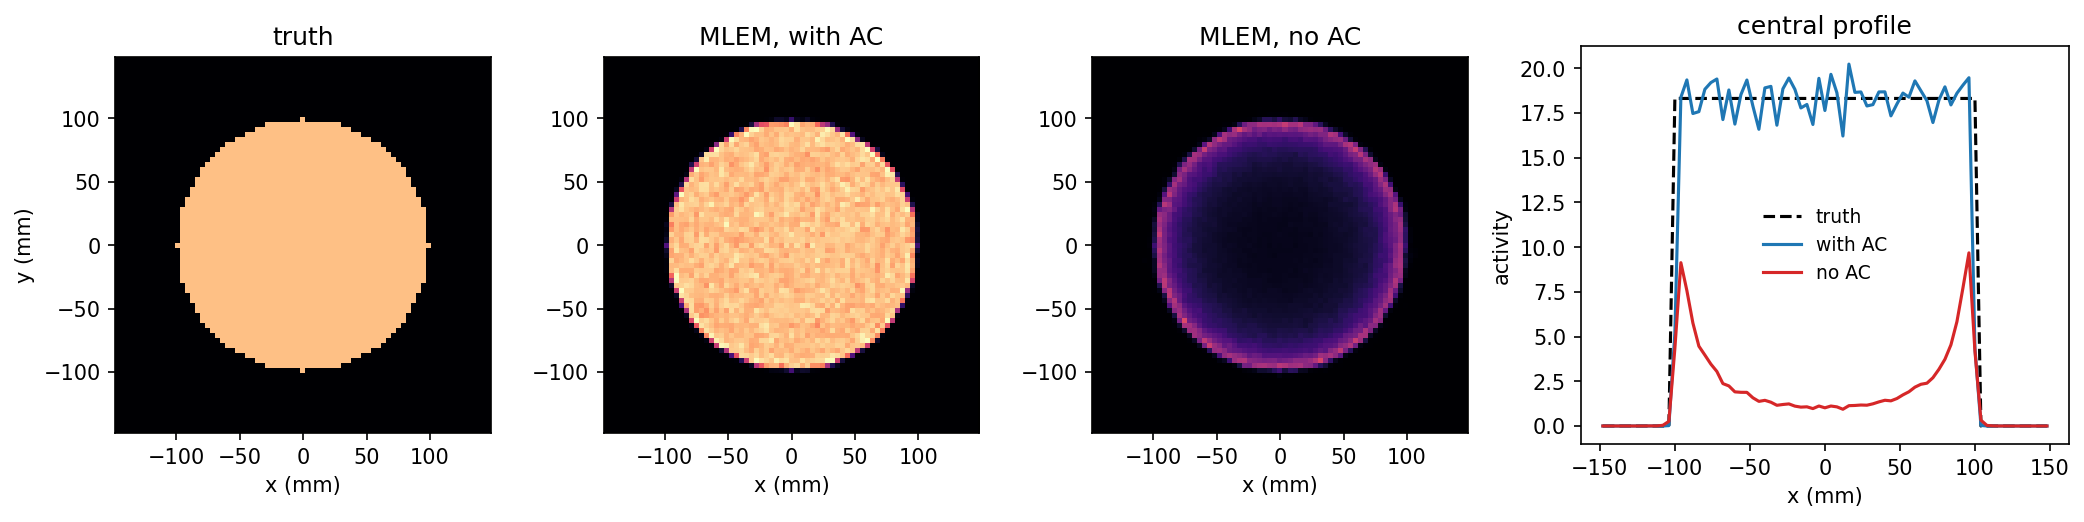
\includegraphics[width=\textwidth]{figures/attenuation_result.png}
  \caption{Uniform water sphere. Central slice of the truth and of the MLEM
    reconstruction with and without attenuation correction (AC), and a central
    profile. Ignoring attenuation cups the image (red); correcting for it
    recovers a flat, quantitative result (blue). Detector resolution is off
    ($\Gop=\mathbf I$), so the only blur is the voxel grid.}
  \label{fig:ex-att}
\end{figure}

The residual graininess in the corrected image is statistical, not bias. It is
controlled here by \emph{early stopping}: MLEM amplifies noise as it iterates
(semi-convergence, Part~I, Acceleration and Noise), and the uniform interior is
already converged by $15$ iterations. Stopping there rather than at $40$ halves
the interior noise (coefficient of variation $0.091\!\to\!0.043$) while slightly
\emph{improving} the relative error --- the extra iterations only amplified
noise. Pushing below this floor would require a smoothness prior (regularization)
rather than more iterations.

\section{Running the example}
\label{sec:ex-att:run}

The code is in \code{tutorial/examples/attenuation/}: \code{run.jl} (simulation
and reconstruction), \code{attenuation.toml} (all parameters), and
\code{attenuation\_plot.py} (the figure). From the repository root:
\begin{lstlisting}
julia --project=tutorial/examples/attenuation -e \
  'using Pkg; Pkg.develop(path="."); Pkg.instantiate()'   # first time
julia -t auto --project=tutorial/examples/attenuation \
  tutorial/examples/attenuation/run.jl
python3 tutorial/examples/attenuation/attenuation_plot.py
\end{lstlisting}
Every number in the figure is reproducible from \code{attenuation.toml}.

\section{What this leaves out}
\label{sec:ex-att:next}

Three physical effects are still switched off and are added in turn in the
following examples: detector \emph{resolution} (the $3.5\,\mathrm{mm}$ Gaussian
$\Gop$ of CRYSP~\cite{crysp2026}), \emph{randoms}, and \emph{scatter}. Each maps
onto the same two library fields as here --- \code{mult} for the multiplicative
factors and \code{contamination} for the additive backgrounds --- so the
reconstruction code does not change; only the simulated data do.

% tbsrc/references.tex — bibliography (self-contained, no bibtex step).
\begin{thebibliography}{9}

\bibitem{joseph1982}
P.~M. Joseph,
\emph{An improved algorithm for reprojecting rays through pixel images},
IEEE Trans.\ Med.\ Imaging \textbf{1}(3):192--196, 1982.

\bibitem{shepp1982}
L.~A. Shepp and Y.~Vardi,
\emph{Maximum likelihood reconstruction for emission tomography},
IEEE Trans.\ Med.\ Imaging \textbf{1}(2):113--122, 1982.

\bibitem{lange1984}
K.~Lange and R.~Carson,
\emph{EM reconstruction algorithms for emission and transmission tomography},
J.\ Comput.\ Assist.\ Tomogr.\ \textbf{8}(2):306--316, 1984.

\bibitem{hudson1994}
H.~M. Hudson and R.~S. Larkin,
\emph{Accelerated image reconstruction using ordered subsets of projection
data},
IEEE Trans.\ Med.\ Imaging \textbf{13}(4):601--609, 1994.

\bibitem{watson2000}
C.~C. Watson,
\emph{New, faster, image-based scatter correction for 3D PET},
IEEE Trans.\ Nucl.\ Sci.\ \textbf{47}(4):1587--1594, 2000.

\bibitem{moses2011}
W.~W. Moses,
\emph{Fundamental limits of spatial resolution in PET},
Nucl.\ Instrum.\ Methods Phys.\ Res.\ A \textbf{648}:S236--S240, 2011.

\bibitem{schramm2024}
G.~Schramm and K.~Thielemans,
\emph{PARALLELPROJ---an open-source framework for fast calculation of
projections in tomography},
Front.\ Nucl.\ Med.\ \textbf{3}:1324562, 2024.

\end{thebibliography}


\end{document}
